\documentclass[a4paper,11pt]{article}
\usepackage[utf8]{inputenc}

% extra packages
% \usepackage{amsrefs}
% \usepackage[autocite=inline,labelalpha=true]{biblatex}

\usepackage[top=1in, left=1in, right=1in, bottom=1in]{geometry}
\usepackage{amsmath, amssymb}
\usepackage{graphicx}
\usepackage{color}
\usepackage{hyperref}

%\setlength{\parindent}{0pt}

\begin{document}

\begin{center}
\Large \textbf{Statement of Research Interests}

\Large Youngmin Park
\end{center}


\section{Introduction}
The main theme of my research is to \textit{advance our understanding of biological systems by using and developing the most effective mathematical tools}. In my research thus far, I use dynamical systems theory as a means to understand neural computation.

\begin{itemize}
 \item \textbf{Park, Y.} and Geffen, M.N. \textit{A Mechanistic Model of the Auditory Cortex with Inhibitory Subtypes} (in preparation). We introduce a groundbreaking model of cortical responses to complex auditory stimuli, which includes inhibitory subtypes implicated in such auditory processing. The model readily generates hypotheses for the role of these inhibitory subtypes across multiple experimental results.

 \item \textbf{Park, Y.}, Shaw, K.M. Chiel, H.J. Thomas, P.J. \textit{The Infinitesimal Phase Response Curve of Oscillators in Piecewise Smooth Dynamical Systems}. European Journal of Applied Mathematics (2018). We provide a first-principles derivation of the phase response curves (PRCs) of oscillators satisfying non-smooth dynamics. This work is a much-needed extension of the half-century-old theory of PRCs.
 
 \item \textbf{Park, Y.}, Ermentrout, G.B. \textit{Weakly Coupled Oscillators in a Slowly Varying World}. (2016). We extend the theory of weakly coupled oscillators to account for a slowly varying parameter, greatly facilitating more realistic and topical studies using dynamic parameters. 
  
 \item \textbf{Park, Y.}, Ermentrout, G.B. \textit{Scalar Reduction of a Neural Field Model with Spike Frequency Adaptation}.
 SIAM Journal on Applied Dynamical Systems (2018). We introduce a novel dimension reduction of so-called ``bump'' solutions of non-local neural field models to centroid coordinates. The dimension reduction allows for a comprehensive analysis of the many bifurcations of the system with greater generality than previously possible.
 
 \item \textbf{Park, Y.}, Ermentrout, G.B. \textit{A Multiple Timescales Approach to Bridging Spiking- and Population-level Dynamics}. (2018). We introduce a powerful theory that robustly accounts for large frequency differences between populations. This substantial contribution enables computational works to operate without the classic restraint of small frequency differences.
 
 \item \textbf{Park, Y.}, Heitmann, S., Ermentrout, G.B. \textit{The Utility of Phase Models in Studying Neural Synchronization}. Book chapter in Computational Models of Brain and Behavior. Wiley-Blackwell (2017). In this book chapter, we explore how different types of phase response curves and synaptic connections affect the synchronization properties of a network. This chapter is the first to address this relationship directly, and provides a much-needed guideline for future computational studies.
 
 \item Shaw, K.M., \textbf{Park, Y.}, Chiel, H.J., Thomas, P.J. \textit{Phase Resetting in an Asymptotically Phaseless System}. SIAM Journal on Applied Dynamical Systems (2012). We derive explicit equations for the phase response curve of a planar, piecewise-linear dynamical system. In contrast to existing beliefs, the work proves that transitions between boundaries can have the greatest effect on the phase response curve.

\end{itemize}



\section{Modeling the Auditory Cortex}
For many decades, modeling studies have sought to reproduce neural responses to simple stimuli, and more recently to temporally complex sounds, such as stimulus-specific adaptation (or deviance detection), and forward suppression (or forward masking). These models robustly reproduce many results, but only include a general inhibitory subpopulation, if any. In particular, they do not account for the latest advancement in neuroscience: optogenetics.

\begin{figure}
\centering
 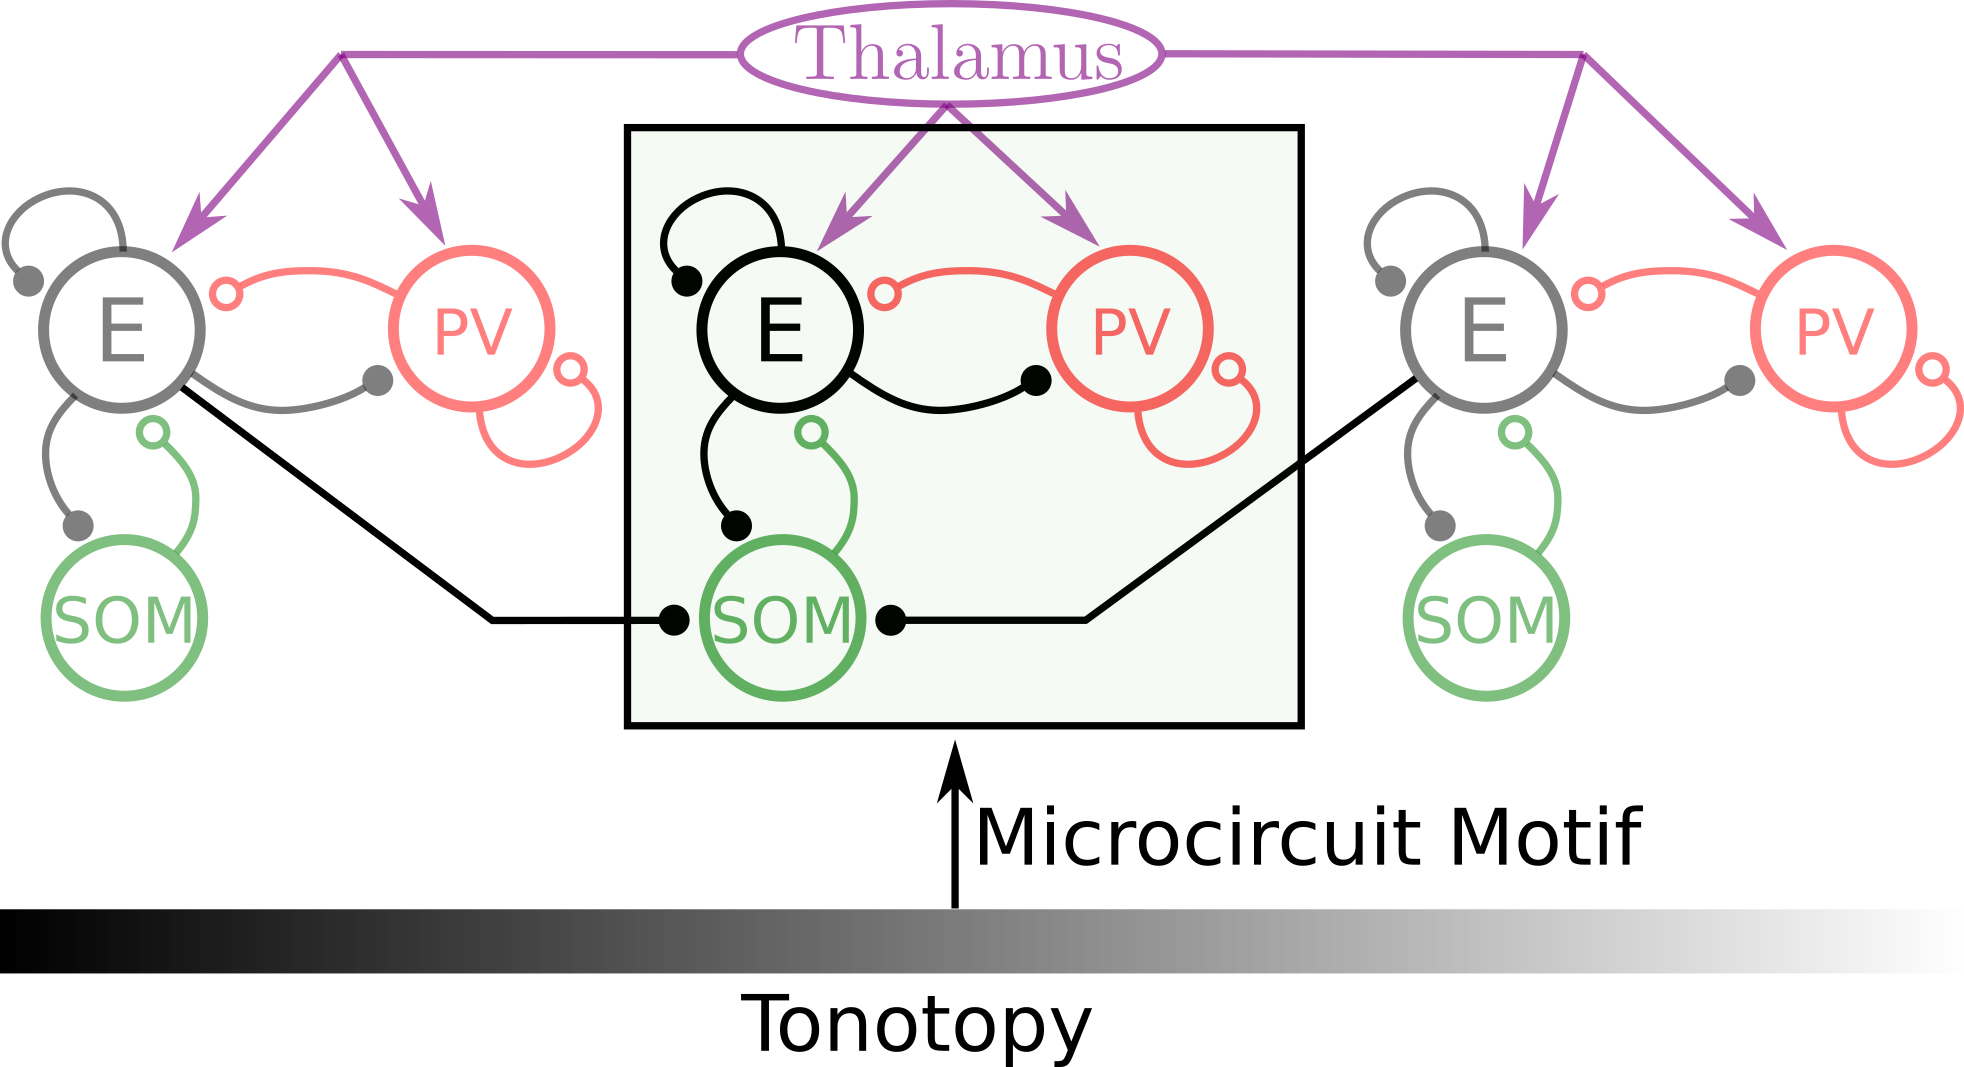
\includegraphics[width=.5\textwidth]{awc.png}
 \caption{A graphical representation of the auditory cortex model. Each circle represents a rate model (Wilson-Cowan dynamics). Pyramidal neurons (E) connect to parvalbumin- (PV, red) and somatostatin-positive (SOM, green) interneurons. The circuit motif consisting of E, PV, and SOM (green square) repeats laterally. Lateral connections exist from E to SOM.}
\end{figure}


Optogenetic techniques allow neuroscientists to selectively activate or inhibit specific inhibitory neuron subtypes with unprecedented temporal precision. Such control allows neuroscientists to study the changes in cortical responses as a function of optogenetic suppression, allowing them to uncover the differential role of interneurons. Models are now being developed to account for such changes in cortical activity, but they are specific to visual cortex \cite{litwin2016inhibitory}, or are relatively abstract and do not generalize well beyond specific results \cite{seybold2015inhibitory,phillips2016asymmetric,phillips2017cortical}.

How the neural circuitry in the auditory cortex produces responses to complex auditory stimuli, and the role of particular interneuron subtypes in shaping these responses remains largely unknown. Thus, our model provides an important advancement of existing studies, and serves as a broawc.pdfad platform to produce additional questions that will further guide ground-breaking experimental studies.

At the moment, the modeling challenge relates to stimulus-specific adaptation (SSA), a phenomenon where neurons respond weakly to a frequent standard tone, but respond strongly to a rare deviant tone at a different frequency. Existing models of SSA use either feedforward inhibition, where synapses adapt to common inputs and remain unadapted to uncommon inputs\cite{mill2011neurocomputational}, or use a lateral propagation of neural activity \cite{yarden2017stimulus}, where deviant tones result in greater lateral propagation than standard tones.

Our approach is two-fold. The first is most like the latter case of lateral propagation where we use a modified Wilson-Cowan model, but in contrast, our method is compatible with existing theoretical results on lateral wave propagation, and do not require additional, computationally-expensive mechanisms (such as population spikes, which describes how neurons in a population typically spike only once during stimulus presentation). One set of interneurons, which we call somatostatin-positive interneurons, provide slow, broad, feedback inhibition, and another set of interneurons, which we call parvalbumin-positive interneurons, provide fast, local, feedforward inhibition. These differential roles appear to reproduce optogenetic results on SSA.

In parallel, we are creating a model in a feedforward scheme, where the auditory inputs have a direct effect on the observed cortical activity (in the case of lateral propagation, auditory inputs do not directly produce the observed cortical activity). In this scheme, the mechanisms are readily understood, and serves to provide an alternative mechanism of SSA, and provides alternative circuitry that can be experimentally tested.

The next step is to establish the parameter range that reproduce results in SSA, and to integrate this result with additional optogenetic studies of temporally-complex stimuli, e.g., tuning-curve adaptation and forward suppression. The model is also compatible with other optogenetic results using simple stimuli, such as constant pure-tones. Interestingly, our current result relies on the network to be in an inhibitory-stabilized state \cite{tsodyks1997paradoxical}, suggesting that primary auditory cortex operates in a similar parameter regime as primary visual cortex.




\section{The Infinitesimal Phase Response Curve of Piecewise Smooth Systems}
Limit-cycle oscillators appear in countless forms in engineering, physics, chemistry, and biology. How large networks of oscillators interact and synchronize is a topic of great interest. The infinitesimal phase response curve (iPRC) quantifies the change in timing due to a small perturbation of a limit cycle trajectory. The iPRC is often a necessary tool for predicting entrainment and synchronization of weakly coupled or weakly forced oscillators. In my masters work with Peter J. Thomas, we extend the classic theory of infinitesimal phase response curves (iPRCs) to the case of planar piecewise smooth dynamical systems \cite{park2013infinitesimal,park2018infinitesimal}, allowing for the application of the theory to a broader class of models.

\begin{figure}
\centering
 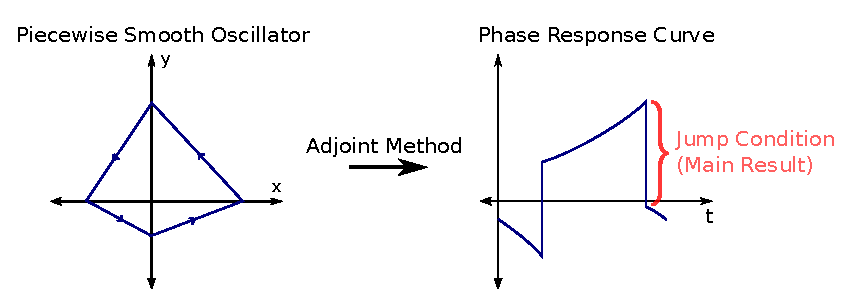
\includegraphics[width=.75\textwidth]{iprc.pdf}
 \caption{Summary of the result. Left: An example of an oscillator satisfying piecewise-smooth dynamics where the switching boundaries coincide with the coordinate axes. Using the classic adjoint method and our jump condition, it is possible to explicitly compute the iPRC including all discontinuities (right). Calculating the size of the discontinuity works in any dimension.}
\end{figure}


For a stable limit cycle in a smooth dynamical system, the iPRC is the gradient $\nabla_x(\theta)$ of the phase function $\theta$\footnote{The asymptotic phase $\theta$ of an initial point $x$ in the stable manifold of a limit cycle identifies the phase of the point on the limit cycle to which the flow $\phi_t(x)$ converges as $t\rightarrow\infty$.}, which can be obtained via the adjoint of the variational equation. For systems with discontinuous dynamics, the standard approach to obtaining the iPRC fails. We derive a formula for the infinitesimal phase response curves (iPRCs) of limit cycles occurring in piecewise smooth (Filipov) dynamical systems of arbitrary dimension, subject to a transverse flow condition. Discontinuous jumps in the iPRC can occur at the boundaries separating subdomains, and are captured by a linear matching condition. The matching matrix, $M$, can be derived from the saltation matrix arising in the associated variational problem. For the special case of linear dynamics away from switching boundaries, we obtain an explicit expression for the iPRC.

% In summary, we find that if the vector field is non-differentiable but continuous, the iPRC has no discontinuities. If the vector field is 

We present popular examples from cell biology (Glass networks) and neuroscience (central pattern generator models). We apply the iPRCs obtained to study synchronization and phase-locking in piecewise smooth limit cycle systems in which synchronization arises solely due to the crossing of switching manifolds. These synchronization results broadly generalize existing coupling literature on piecewise smooth systems, which are often restricted to one or a combination of linear coupling, planar systems, and piecewise linear vector fields \cite{coombes2016synchrony,izhikevich2000phase,coombes2012nonsmooth}.


This work establishes an important link between the saltation matrix, a correction term for forward-time solutions of non-smooth systems, and our matching condition, which is a correction term for solutions in backwards-time of non-smooth systems. This relationship reveals that advanced results using the saltation matrix may apply in the case of the phase response curve. A natural next step will be to establish the conditions for weakly coupled oscillators of non-smooth systems.


\section{Synchronization of Weakly Coupled Oscillators Modulated by a Slowly Varying Parameter}
Local neural circuits may be modulated by slowly varying concentrations of neuromodulators. These slow modulations may change a few parameters by small amounts, yet result in drastic effects on the synchronization properties of coupled oscillators. Understanding how these changes happen is the subject of our first paper \cite{park2016weakly}.

To this end, we extend the theory of weakly coupled oscillators to incorporate a slowly varying input. In contrast to the derivation of the classic theory, which uses averaging, we employ a combination of regular perturbation and an adiabatic approximation to derive differential equations for the phase-difference between a pair of oscillators. This method works so long as the parameter varies slowly (with no restrictions on amplitude), the coupling is weak, and the limit cycle solution persists for all parameter values. The derivation naturally extends to an arbitrary number of coupled oscillators that are each modulated by the same parameter. 

We apply this theory to several example models. The first model is a simple Hopf oscillator, where the parameter modulates the angular frequency for solutions perturbed away from the limit cycle attractor. As the parameter varies, it modulates the shape of the phase response curve, changing it in both amplitude and sign. These changes result in different synchronization properties between two Hopf oscillators. We also consider weak (order $\varepsilon$ small) heterogeneities and show great agreement between our reduction method and the full numerical simulations.

The second model is a conductance-based biophysical model of an excitatory cortical neuron, where the slowly varying parameter modulates one conductance. This setup represents the behavior of a neuron that is subject to slow modulation of a muscarinic current such as would occur during transient attention through cholinergic activation. Strikingly, small changes to this parameter results in drastic changes to the PRC, resulting in different synchronization properties as the parameter varies. In addition to the simple case of two neurons with reciprocal excitatory coupling, we apply the method to an all-to-all excitatory network and show that there is a waxing and waning of synchrony of modulated neurons.

In all examples, we use slowly varying parameters that are periodic, quasi-periodic, and stochastic (an Ornstein-Uhlenbeck process with slow drift).

The neural examples used excitatory cortical models, but the framework is powerful enough to account for inhibitory interneurons as well as inhibitory subtypes. How these inhibitory subtypes modulate phase response curves in addition to an external neuromodulator will be a fruitful next step.

% The first project to exploit multiple timescales was on the synchronization of conductance-based neural models modulated by a slowly varying level of acetylcholine. This separation of timescales allowed for a phase reduction and a standard weak coupling analysis \cite{park2016weakly}.

\section{Spatio-Temporal Dynamics of a Bump Solution of a Neural Field Model}
Neural field models are an immensely valuable tool for understanding how the brain operates at the population-level. Neural field models are capable of generating numerous spatio-temporal patterns, including traveling waves and pulses \cite{coombes_bumps_2005}, and solutions of neural fields have been proposed as mechanisms of neural processing in the mammalian neocortex \cite{itskov_2011_cell,folias2011nonlinear,pinto_ermentrout_2001_siam}.

\begin{figure}
\centering
 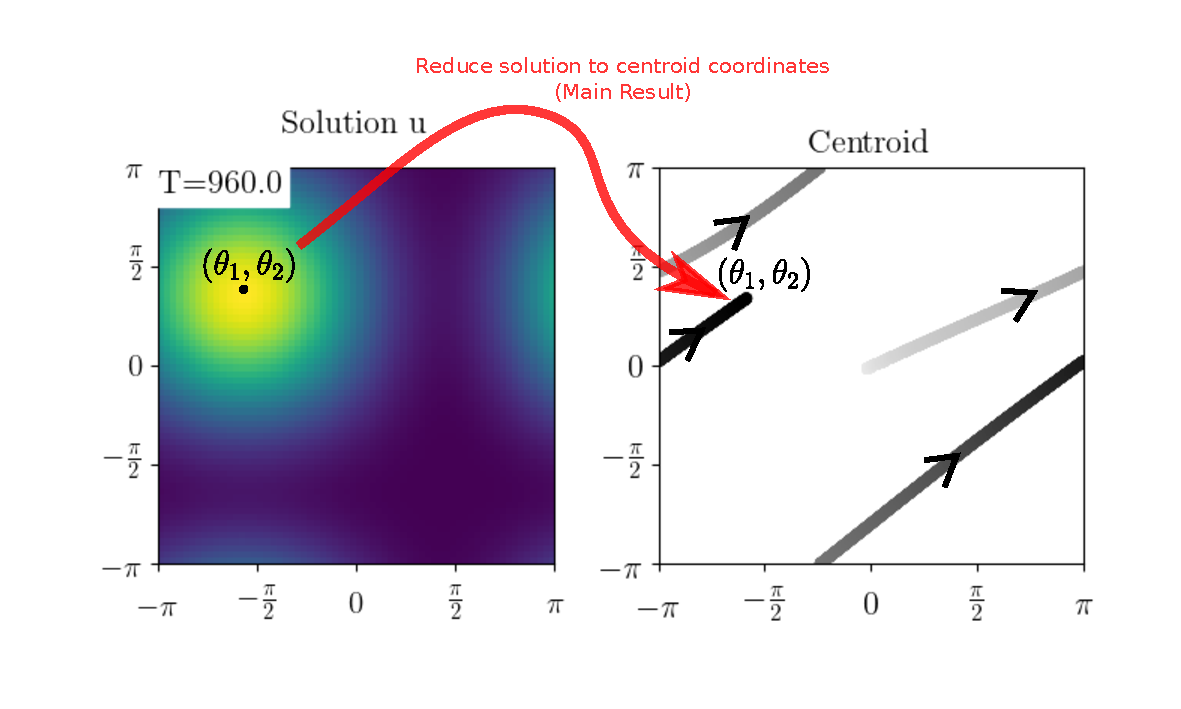
\includegraphics[width=.75\textwidth]{bump.pdf}
 \caption{The reduction of the bump solution to centroid coordinates. Left: The bump solution after 960 time units. Lighter colors represent high neural activity, while darker colors represent low neural activity. Right: The trace of the centroid position over time, where lighter tones represent old positions, and darker tones represent recent positions. The key idea of this result is the reduction from the full solution (left) to a pair of reduced equations of the centroid (right).}
\end{figure}

In this project, we analyze a particular neural field model, first studied in \cite{pinto_ermentrout_2001_siam}, with weak and slow spike-frequency adaptation, and weak, spatially localized inputs \cite{park2018scalar}. While neural field models are capable of producing a vast number of spatio-temporal patterns \cite{breakspear2017dynamic}, we consider the special case of a single ``bump'' solution, which is loosely defined as a spatially coherent region of activity. This bump exhibits slow timescale translational movement dependent on the strength of the input and adaptation.

The weak and slow interactions allow us to consider a separation of timescales between the fast recurrent network activity that results in the bump, and the slow timescale of adaptation. As part of the regular perturbation we include terms to account for the slow timescale shifts in the centroid of the bump solution, thus reducing the infinite dimensional partial integro-differential equation to a system of two scalar delay integro-differential equations.

For the remainder of the paper, we determine the existence and stability of the many spatio-temporal solutions of the bump solution, using the scalar delay equations. One the ring, we show the existence and stability of different motions including constant-velocity, non-constant velocity, and oscillations. We use a combination of analytical methods, as the delay equations are analytically tractable, as well as a slew of numerical methods, such as XPPAUTO\cite{xpp}, to confirm the analytical results.

On the torus, we show a similar set of results. In this case, the analysis of the full simulation are almost entirely intractable for the tools available to us. It is in this case we demonstrate the power of our dimension reduction, and generate detailed bifurcation diagrams of the spatio-temporal dynamics with relative ease. Moreover, we compute similar results as in the ring domain, showing existence and stability of constant and non-constant velocity solutions, as well as the existence of oscillations.

In addition to the tractability of this reduction, we introduce generalizations not present in existing studies. For instance, we do not use non-smooth assumptions like the high-gain limit of the firing rate function. At the same time, we allow the synaptic connectivity profile to be general, so long as the connectivity admits a bump solution.

Any neural field model that produces a simple, structurally coherent pattern with some weak and slow dynamics are excellent candidates for this reduction analysis. For example, traveling waves with some sufficiently slow variables could be amenable to a multiple timescale analysis, where the reduced dynamics could describe the velocity of the wave and the direction of the wave front on a two dimensional domain. A similar approach could be used to reduce the dimensionality of spiral waves, which are often used to model epileptic seizures.

\section{The Connection Between the Mean-Field Description and Spiking Neurons}

The original derivation of the Wilson-Cowan model did not begin at the spiking-level, but instead opted for general macroscopic quantities such as the probability of neurons to fire. This often-called ``phenomenological'' description was satisfactory for decades, due in part to the success of the model as a mechanistic framework of the cortex. In more recent decades, researchers have returned to the starting point and are starting to derive the mean-field equations from spiking models. The approach diverges at the start, where one group requires total asynchrony \cite{laing2014derivation,laing_exact_2015,renart2007mean} and Poisson statistics \cite{amit1997model,amit1997dynamics}, while the other group requires information about synchrony at the population-level \cite{coombes2016next,so2008synchronization}. Our work fits in with the latter case, where we seek to derive phase equations for the population.

Extending upon our first paper, we rigorously determine the effects of internally-generated slow processes that in turn modulate the system \cite{park2018multiple}. We consider a system of all-to-all synaptically coupled oscillators, where the averaged synaptic dynamics operate on a much slower timescale. That is, while the synaptic variable my change instantaneously due to a presynaptic spike, this effect is small in amplitude, and with enough presynaptic spikes over enough time, the average value of the synaptic variable may vary on a slow timescale. For convenience we call these synapses ``slow''.

Such a set up allows the synaptic variables to operate in agreement with mean-field dynamics. If $s^x$ ($s^y$) is the synapse for the excitatory (inhibitory) population, then their averaged values $\bar s^x$ ($\bar s^y$) each satisfy ordinary differential equations with right-hand sides that depend on the frequency of each population. These equations already represent a reduced system, however, they contain no information about the degree of synchrony of the population. The mean-field synaptic variables may exhibit non-trivial dynamics, such as oscillations, which in turn affect the spiking-level synchronization as observed by numerical simulations.

The separation of timescales between the neural oscillations and the slow synapses allows for a dimension reduction similar to that of the first paper, and we derive a system of phase equations that allow us to determine phase differences between the oscillators. Roughly speaking, we transform the strong, slow synaptic coupling into weak, fast coupling, which is then a weakly coupled system amenable to the classic phase reduction \cite{rubinrubin}. However, the synaptic variables may vary away from some fixed point, so we include an additional term into the derivation, which accounts for this case.

As a result of this additional term, our phase reduction accounts for the cases of large phase drift caused by small and slow oscillations in the mean synaptic variables. This striking result extends classic work on weak coupling theory, which requires all oscillators to have the same frequency, or small differences in frequencies. In an interesting twist, our phase reduction includes the mean-field synapses as external inputs. That is, suppose we compute the population-averaged dynamics of a system satisfying our assumptions. The averaging process may have destroyed information about synchrony at the spiking-level. However, by placing the averaged dynamics into our reduction, it is possible to predict spiking-level synchrony. Thus, our work also serves as a proof-of-concept that in some cases, spiking-level information is preserved even after averaging.

We apply this method to several cases. The first case includes theta models \cite{ek84} with heterogeneities in the synaptic inputs. The second case includes a network of excitatory Traub models \cite{traub1982simulation} and inhibitory Wang-Buzs{\'a}ki model \cite{wang1996gamma}. In all cases we find robust agreement between theory and numerics. In some cases, the dynamics are sufficiently simple to allow for analytical calculation, and we also show the existence and stability of various phase-locked solutions.

Our examples are one of the first nontrivial extensions of existing studies that consider only one-dimensional dynamics. Our theory is much greater in scope, accounting for more complex coupling such as as first-order (or greater) chemical synapses, and is robust to greater heterogeneities in more complicated models.

As a next step, we will account for the case where these equations become more complex as the population grows. How to derive a population-level measure of synchrony, e.g., the order parameter, is of great interest.

\section{Phase Resetting in an Asymptotically Phaseless System: On the Phase Response of Limit Cycles Verging on a Heteroclinic Orbit}

Animals often generate reliable sequences of motor actions, such as breathing, walking, and swimming. How animals modulate these robust rhythms is largely an open question. One possible class of models for such sequential activity includes heteroclinic cycles. A dynamical system possess a heteroclinic sequence if there exists a chain of hyperbolic saddle fixed points for which the unstable manifold of each saddle intersects the stable manifold of the next \cite{shaw2012phase}.

Such a configuration has the practical effect of ``dwell times'', where a trajectory close to the heteroclinic cycle will pass each saddle point with low velocity. Such a system mimics, for example, the feeding pattern of \textit{Aplysia Californica}, where the feeding apparatus dwells in discrete states. Interestingly, the dwell times of these states increase as a function of reduced proprioceptive feedback, which is indicative of an oscillatory system that traverses closer and closer to a heteroclinic cycle (as a function of some bifurcation parameter) \cite{shaw2010evidence}.

By considering a planar piecewise-linear system admitting a limit-cycle solution and a heteroclinic bifurcation, we manage to derive, explicitly, the infinitesimal phase response curve (iPRC) of this system. This derivation is significant for several reasons. One, it is one of the few explicitly computable iPRCs in existence. Two, the derivation proved that the sensitivity of the iPRC is greatest as the limit-cycle solution crosses the boundary between piecewise regions (which, incidentally, is the point farthest from any saddle points). The latter result is a striking contradiction to assumptions taken in earlier studies, where it was assumed that the most important times are where the limit cycle passes within a small neighborhood of saddle points \cite{brown2004phase}.

The next step is to map these results back to a realistic biological central pattern generator. Precisely how the central pattern generator is modulated, how it is modulated, and the amount of energy expended for modulation are important questions. An important theoretical question is to understand how general limit cycles near heteroclinic cycles use less energy to control than limit cycles that do not emerge from a heteroclinic bifurcation.

% \subsection{General Weakly Coupled Piecewise Smooth Oscillators}
% In addition to these primary studies, I have continued to build on my masters work in continued collaborations with my masters thesis advisor Peter J. Thomas (with colleagues Hillel J. Chiel and Kendrick M. Shaw). We generalized the result of my masters thesis to $n$-dimensions and applied the result to weakly coupled piecewise smooth systems \cite{park2016infinitesimal}. Most existing literature on coupling of piecewise smooth systems are often restricted to one or a combination of linear coupling, planar systems, and piecewise linear vector fields \cite{coombes2016synchrony,izhikevich2000phase,coombes2012nonsmooth}. Although we required solutions to be continuous, our weak coupling analysis applies to piecewise smooth systems of arbitrary dimension with nonlinear, heterogeneous coupling \cite{park2018infinitesimal}.

\section{Worcester Polytechnic Institute}

My research experience perfectly complements existing research at Worcester. I seek to build an understanding of interactions between neurons, and the effects of internal and external modulators on these interactions. This type of work exhibits parallels with research interests of current faculty, for instance, Sarah Olson's extensive work on fluid-structure interactions and calcium dynamics. I identify her as a potential collaborator and mentor, as her work directly aligns with my future research goals to pivot into different arenas of biology. In addition, I identify Zhongqiang Zhang as another potential collaborator and mentor, as my work on non-smooth systems aligns with his research on fractional differential equations and non-smooth systems.

\bibliographystyle{alpha}
\bibliography{../../youngmin-bard/bio,../../youngmin-bard/neuralfield,../../youngmin-bard/math,../../youngmin-bard/phase,../../youngmin-bard/computation,../../youngmin-bard/cortex}


\end{document}
